\chapter{Mathematical models of Bose-Einstein condensates}\label{chap: theory}

In this chapter we provide the theoretical background necessary to understand
the dynamics of ultracold atomic gases.
We begin by introducing the most simple form of a BEC, the scalar condensate.
This lays the framework for building to more complex systems.
We then go on to discuss the two-component condensate, where additional
interactions arise between atoms of differing components.
Finally, we construct the framework needed to understand spinor BECs, which is
the main focus of this thesis.

\section{Mean-field description of scalar condensates}
Consider a system of bosons which is dilute enough such that we may approximate
interactions between bosons as two-body interactions only.
Such a system is described by the Hamiltonian~\cite{Pitaevskii2003}
\begin{align}\label{eq: scalar-hamiltonian}
    \hat{H} = \hat{H}_0 + \hat{H}_I.
\end{align}
Here, \(\hat{H}_0\) is the single-particle Hamiltonian:
\begin{align}
    \hat{H}_0 = \int \hat{\Psi}^\dagger(\vb{r}, t)\left[
        -\frac{\hbar^2\nabla^2}{2m} + V(\vb{r}, t)
    \right]\hat{\Psi}(\vb{r}, t)\, \dd^3\vb{r},
\end{align}\
where \(\hat{\Psi}(\vb{r}, t)\) is the field operator that annihilates a boson
at position \(\vb{r}\) at time \(t\).
The first term represents the kinetic energy operator and \(V(\vb{r}, t)\)
is a trapping potential.
Additionally, \(\hat{H}_I\) represents the interacting part of the Hamiltonian,
which describes binary collisions between bosons at positions \(\vb{r}_1\) and
\(\vb{r}_2\) whose interactions are described by the interaction potential
\(\mathcal{U}(\vb{r}_1, \vb{r}_2)\):
\begin{align}
    \hat{H}_I = \frac{1}{2}\int \int \hat{\Psi}^\dagger(\vb{r}_1, t)
    \hat{\Psi}^\dagger(\vb{r}_2, t)\mathcal{U}(\vb{r}_1, \vb{r}_2)
    \hat{\Psi}(\vb{r}_2, t)\hat{\Psi}(\vb{r}_1, t)
    \, \dd^3\vb{r}_1 \, \dd^3\vb{r}_2.
\end{align}
The dilute nature of the BEC justifies that any binary interaction
between two particles at positions \(\vb{r}_1, \vb{r}_2\) can be approximated by
a contact interaction modelled by the following delta function:
\begin{equation}
    \mathcal{U}(\vb{r}_1, \vb{r}_2) = g\delta(\vb{r}_1 - \vb{r}_2),
\end{equation}
where the interaction coefficient, \(g\), is related to the s-wave scattering
length, \(a_s\), as
\begin{align}\label{eq: scalar-interaction-coeff}
    g = \frac{4\pi\hbar^2a_s}{m},
\end{align}
for a boson with atomic mass \(m\).

\subsection{The Gross-Pitaevskii equation}
The Heisenberg picture states that the time evolution for the field operator
\(\hat{\Psi}(\vb{r}, t)\) is given by~\cite{Pitaevskii2003}
\begin{align}
    i\hbar\pdv{\hat{\Psi}(\vb{r}, t)}{t} = \left[\hat{\Psi}(\vb{r}, t), \hat{H}
    \right],
\end{align}
which, using Eq.~\eqref{eq: scalar-hamiltonian}, is calculated to be
\begin{align}\label{eq: scalar-field-operator-motion}
    i\hbar\pdv{\hat{\Psi}(\vb{r}, t)}{t} = \left[-\frac{\hbar^2\nabla^2}{2m}
    + V(\vb{r}, t)\right]\hat{\Psi}(\vb{r}, t)
    + g\hat{\Psi}^\dagger(\vb{r}, t)\hat{\Psi}(\vb{r}, t)\hat{\Psi}(\vb{r}, t).
\end{align}
Now, since we consider a system close to absolute zero, we make the assumption
that most atoms occupy the same quantum state, and hence we can decompose the
field operator into a mean and fluctuation parts as~\cite{Pitaevskii2003}
\begin{align}
    \hat{\Psi}(\vb{r}, t) = \psi(\vb{r}, t) + \delta\hat{\psi}(\vb{r}, t),
\end{align}
where \(\psi \equiv \langle \hat{\Psi}(\vb{r}, t)\rangle\) is a classical scalar
field describing the wave function of the condensate, which describes the
spatially-coherent condensed state.
Here, \(\delta\hat{\psi}(\vb{r}, t)\) describes deviations from this mean and
\(\langle \delta\hat{\psi}(\vb{r}, t)\rangle = 0\).
Substituting the above form of the field operator into
Eq.~\eqref{eq: scalar-field-operator-motion}, taking the expectation and
ignoring terms of \(\delta\hat{\psi}^2\) or higher yields the equation of motion
for the wave function of a Bose-Einstein condensate, the Gross-Pitaevskii
equation (GPE):
\begin{equation}\label{eq: scalar-GPE}
    i\hbar \pdv{\psi(\vb{r}, t)}{t} = \left(-\frac{\hbar^2}{2m}\nabla^2
    + V(\vb{r}, t) +g|\psi(\vb{r}, t)|^2\right)\psi(\vb{r}, t).
\end{equation}
Neglecting the fluctuation terms is only valid when considering a system at zero
temperature, where there are no contributions from thermal fluctuations and
contributions from quantum fluctuations are negligible in comparison to the
classical field.

For \(g>0\) the interactions are repulsive and for \(g < 0\) they are
attractive.
When \(g=0\) there are no interactions present and the system reduces to the
Schr\"{o}dinger equation.
The wave function of the system is normalised to the number of particles
\begin{equation}
    \int |\psi(\vb{r}, t)|^2 \, \dd^3\vb{r} = N,
\end{equation}
which remains conserved under the GPE\@.
Finally, the total energy of the system is given by
\begin{equation}\label{eq: scalar-energy}
    E = \int  \left[\frac{\hbar^2}{2m}|\nabla\psi(\vb{r}, t)|^2
        + V(\vb{r}, t)|\psi(\vb{r}, t)|^2 + \frac{g}{2}|\psi(\vb{r}, t)|^4
        \right] \, \dd^3\vb{r}
    = E_\text{kin} + E_\text{pot} + E_\text{int},
\end{equation}
where \(E_\text{kin}, E_\text{pot}\) and \(E_\text{int}\) describes the
kinetic, potential, and interaction energies, respectively.

\section{Two-component Bose-Einstein condensates}\label{sec: two-comp-theory}
We now generalise part of the theory introduced in the previous section to
describe multi-component condensates.
The time-dependent coupled Gross-Pitaevskii equations each describe a condensate
similar to the standard GPE given in Eq.~\eqref{eq: scalar-GPE}, but now with an
additional non-linear term that describes the interactions of atoms between
condensate components.
The coupled GPEs are given as
\begin{equation}\label{eq: two-component-GPEs}
    \begin{aligned}
        i\hbar \pdv{\psi_1(\vb{r}, t)}{t} & =
        \left[-\frac{\hbar^2}{2m_1}\nabla^2 + V_1(\vb{r}, t)
            + g_1|\psi_1(\vb{r}, t)|^2
        + g_{12}|\psi_2(\vb{r}, t)|^2\right]\psi_1(\vb{r}, t), \\
        i\hbar \pdv{\psi_2(\vb{r}, t)}{t} & =
        \left[-\frac{\hbar^2}{2m_2}\nabla^2 + V_2(\vb{r}, t)
            + g_2|\psi_2(\vb{r}, t)|^2
            + g_{12}|\psi_1(\vb{r}, t)|^2\right]\psi_2(\vb{r}, t),
    \end{aligned}
\end{equation}
where \(\psi_j(\vb{r}, t)\) corresponds to the wave function of component \(j\)
with atomic mass \(m_j\) for \(j=1, 2\), and \(V_j(\vb{r}, t)\) is an external
trapping potential.
The interaction terms are a generalised from of
Eq.~\eqref{eq: scalar-interaction-coeff}, given explicitly as
\begin{equation}
    g_j = \frac{4\pi \hbar^2a_j}{m_j}, \qquad
    g_{12} = \frac{2\pi\hbar^2(m_1+m_2)a_{12}}{m_1m_2},
\end{equation}
which describe the intraspecies and interspecies interaction strengths,
respectively.
Similar to the scalar case, the wave function of each component is normalised
to the number of atoms of that component
\begin{equation}
    \int |\psi_j|^2 d^3\vb{r} = N_j.
\end{equation}

The time-independent GPEs can be obtained by making the following substitution
of the wave function \(\psi_j(\vb{r}, t)=\psi_j(\vb{r})e^{-i\mu_j t/\hbar}\) in
Eq.~\eqref{eq: two-component-GPEs}, yielding
\begin{equation}\label{eq: time-indep-two-component-GPEs}
    \begin{aligned}
        \mu_1\psi_1(\vb{r}) & =
        \left[-\frac{\hbar^2}{2m_1}\nabla^2 + V_1(\vb{r})
            + g_1|\psi_1(\vb{r})|^2
        + g_{12}|\psi_2(\vb{r})|^2\right]\psi_1(\vb{r}), \\
        \mu_2\psi_2(\vb{r}) & =
        \left[-\frac{\hbar^2}{2m_2}\nabla^2 + V_2(\vb{r})
            + g_2|\psi_2(\vb{r})|^2
            + g_{12}|\psi_1(\vb{r})|^2\right]\psi_2(\vb{r}),
    \end{aligned}
\end{equation}
where \(\mu_j\) is the chemical potential of component \(j\).
The total energy of the two-component system comprises the same contributions to
the energy as the scalar case given in Eq.~\eqref{eq: scalar-energy}, i.e.,
\(E = E_\text{kin} + E_\text{pot} + E_\text{int}\), but with contributions from
both components as
\begin{equation}
    \begin{aligned}
        E & = \int \left[\frac{\hbar^2}{2m_1}|\nabla\psi_1|^2
        + V_1(\vb{r})|\psi_1|^2 + \frac{g_1}{2}|\psi_1|^4 \right] \dd^3\vb{r} \\
          & + \int \left[\frac{\hbar^2}{2m_2}|\nabla\psi_2|^2
        + V_2(\vb{r})|\psi_2|^2 + \frac{g_2}{2}|\psi_2|^4 \right] \dd^3\vb{r} \\
          & + \int \left[g_{12}|\psi_1|^2|\psi_2|^2\right] \dd^3\vb{r}.
    \end{aligned}
\end{equation}

\subsection{Miscible and immiscible regimes}
Two-component condensates can be either miscible or immiscible, depending on
the interactions present within the system.
Here, we derive the immiscibility criterion for two-component condensates
following the procedure in Ref.~\cite{Ao1998}.
We start by assuming, for simplicity, a BEC in the absence of a trapping
potential such that \(V_1(\vb{r}) = V_2(\vb{r}) = 0\).
Assuming a homogeneous stationary solution where the kinetic energy terms can
be neglected, Eq.~\eqref{eq: time-indep-two-component-GPEs} reduces to
\begin{equation}
    \begin{aligned}
        \mu_1 & = g_1|\psi_1|^2 + g_{12}|\psi_2|^2, \\
        \mu_2 & = g_2|\psi_2|^2 + g_{12}|\psi_1|^2.
    \end{aligned}
\end{equation}
Let us consider a miscible regime, where, inside the trap, the densities of each
component can be re-written as \(n_j=N_j/\mathcal{V}\), where \(\mathcal{V}\) is
the volume of the condensate.
The above equations then reduce to \(g_1n_1 + g_{12}n_2 = \mu_1\) and
\(g_2n_2 + g_{12}n_1 = \mu_2\), and the energy becomes
\begin{equation}
    E_\mathrm{misc} = \frac{1}{2}\left[g_1\frac{N_1^2}{\mathcal{V}}
    + g_2\frac{N_2^2}{\mathcal{V}} + 2g_{12}\frac{N_1N_2}{\mathcal{V}}\right].
\end{equation}
Provided \(g_{12}\) is small enough, any variation to this state will increase
the system energy, implying that this state is stable.
When \(g_{12}\) gets large enough, however, it can be shown that there exists
a state with a lower energy.

Let us consider an immiscible regime, where the two condensates do not spatially
overlap.
The volume of condensate \(j\) is given as \(\mathcal{V}_j\) and the densities
subsequently become \(n_j=N_j/\mathcal{V}_j\).
Assuming that the contribution to the energy arising from the interface between
the two condensates is negligible in comparison to the contribution from the
bulk, Eqs.~\eqref{eq: time-indep-two-component-GPEs} reduce to
\(g_j n_j = \mu_j\) with the total energy
\begin{equation}\label{eq: immiscible-energy}
    E_\mathrm{immisc} = \frac{1}{2}\left[g_1\frac{N_1^2}{\mathcal{V}_1}
        + g_2\frac{N_2^2}{\mathcal{V}_2}\right].
\end{equation}
Minimising the above energy with respect to \(\mathcal{V}_1\) or
\(\mathcal{V}_2\) with \(\mathcal{V}=\mathcal{V}_1+\mathcal{V}_2\) results in
the expressions for the volume of each component
\begin{equation}
    \mathcal{V}_1 = \frac{1}{1 + \sqrt{g_2/g_1}(N_2/N_1)}\mathcal{V},
\end{equation}
\begin{equation}
    \mathcal{V}_2 = \frac{1}{1 + \sqrt{g_1/g_2}(N_1/N_2)}\mathcal{V}.
\end{equation}
The corresponding densities then become
\begin{equation}
    \begin{aligned}
        n_1 = \left(1 + \sqrt{\frac{g_2}{g_1}}\frac{N_2}{N_1}\right)
        \frac{N_1}{\mathcal{V}}, \quad
        n_2 = \left(1 + \sqrt{\frac{g_1}{g_2}}\frac{N_1}{N_2}\right)
        \frac{N_2}{\mathcal{V}}.
    \end{aligned}
\end{equation}
Substituting the above densities into the expression for the total energy
in Eq.~\eqref{eq: immiscible-energy} yields
\begin{equation}
    E_\mathrm{immisc} = \frac{1}{2}\left[g_1\frac{N_1^2}{\mathcal{V}}
    + g_2\frac{N_2^2}{\mathcal{V}}
    + 2\sqrt{g_1g_2}\frac{N_1N_2}{\mathcal{V}}\right],
\end{equation}
and the difference between the energies of the miscible and immiscible phases is
subsequently calculated as
\begin{equation}
    \Delta E = E_\mathrm{misc} - E_\mathrm{immisc} = (g_{12} - \sqrt{g_1g_2})
    \frac{N_1N_2}{\mathcal{V}}.
\end{equation}
Therefore, the condition \(g_{12} > \sqrt{g_1g_2}\) reveals that for large
enough interspecies interactions the system favours an immiscible phase
over a miscible one.
This criterion only depends on the interactions within the system, and is not
affected by condensate particle numbers or size.
Fig.~\ref{fig: miscible-vs-immiscible} shows the boundary between the two
phases for \(g_1=1\) in a parameter space of \(g_2, g_{12}\).
\begin{figure}
    \centering
    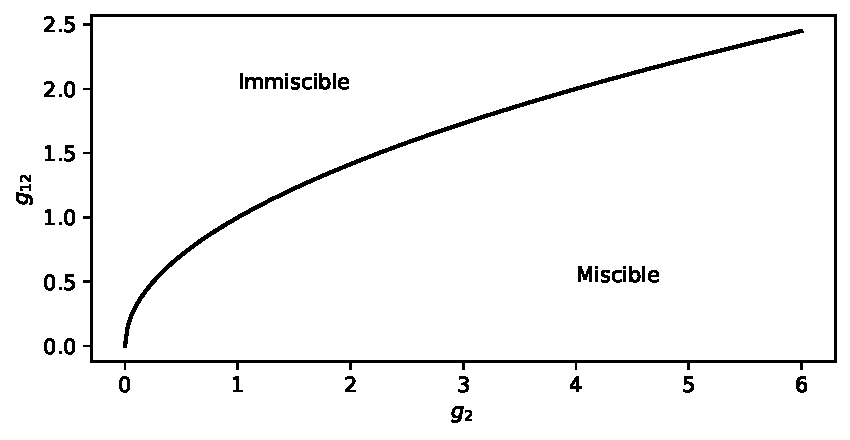
\includegraphics{gfx/ch-theory/miscible_vs_immiscible.pdf}
    \caption[Two-component miscible vs immiscible boundary]
    {\label{fig: miscible-vs-immiscible}Boundary between the miscible
        and immiscible regimes for a two-component condensate with \(g_1=1\).}
\end{figure}


\section{Spinor Bose-Einstein condensates}
Spinor systems are comprised of particles with total hyperfine spin \(f\).
The hyperfine spin is made up of contributions from the atoms' electron spin,
\(s\), the electron orbital angular momentum, \(l\), and the nuclear spin,
\(i\)~\cite{Kawaguchi2012}.
Canonical examples include \(^{23}\)Na and \(^{87}\)Rb, which can be realised as
both \(f=1\) and \(f=2\) systems, and \(^{52}\)Cr, which can be realised as an
\(f=3\) system.
A hyperfine spin \(f\) implies that there are \(2f + 1\) possible spin states
along a given spin quantisation axis.
Such a state is denoted \(\ket{f, m} \), where
\(m \in \{-f, -f+1, \ldots, 0, \ldots, f - 1, f\} \) denotes the magnetic
sublevel for an atom with total spin \( f\).
A system of identical spin-\(f\) bosons is described by the field operators
\(\hat{\psi}_m(\vb{r})\) which satisfy the following commutation
relations~\cite{Kawaguchi2012}:
\begin{align}
    \left[\hat{\psi}_m(\vb{r}_1), \hat{\psi}^\dagger_{m'}(\vb{r}_2)\right]
    &= \delta_{mm'}\delta(\vb{r}_1 - \vb{r}_2), \\
    \left[\hat{\psi}_m(\vb{r}_1), \hat{\psi}_{m'}(\vb{r}_2)\right] &=
    \left[
        \hat{\psi}^\dagger_m(\vb{r}_1), \hat{\psi}^\dagger_{m'}(\vb{r}_2)
    \right] = 0.
\end{align}
To construct the relevant spinor Hamiltonians we follow the methodology in
Refs~\cite{Ho1998,Ohmi1998,Kawaguchi2012,Stamper-Kurn2013,Symes2019} and make
the following assumptions: We assume only elastic and binary collisions between
atoms, implying that the total spin is conserved, as well as low incident
collision energy so that only s-wave scattering is observed.
Additionally, we assume no spin-orbit coupling and no mixing of
hyperfine states.

\subsection{Contributions from spin-channels}
Collisions between two incoming spin-\(f\) atoms in magnetic sublevels \(m\)
and \(m'\) can undergo spin-exchange interactions, where the outgoing particles
can now be in entirely different magnetic sublevels.
In the case of s-wave scattering, where the orbital angular momentum is zero,
\(\EuScript{M} \equiv m + m'\) is conserved~\cite{Kawaguchi2012}.
For example, collisions between two spin-1 atoms located in sublevels \(m=1\)
and \(m'=-1\) must collide to form \(\EuScript{M} = 0\), implying that the only
allowed exchange is:
\begin{align}\label{eq: spin-1-exchanges}
    (1, -1) \leftrightarrows (0, 0).
\end{align}

In general, a collision between two spin-\(f\) atoms can combine to have a total
spin \(\EuScript{F} \in \{0, 1, \ldots, 2f\}\) and
\(\EuScript{M} \equiv m + m' \in \{-\EuScript{F}, \ldots, \EuScript{F}\}\).
In the s-wave scattering limit, the total spin \(\EuScript{F}\) of two colliding
atoms must be a multiple of \(2f\), i.e., \(\EuScript{F} \in
\{0, 2, \ldots, 2f\}\), since the wave function must remain symmetric under the
exchange of the two atoms~\cite{Pethick2008}.
The total interaction Hamiltonian is constructed as a sum of each
contribution from individual spin channels as~\cite{Kawaguchi2012}
\begin{align}\label{eq: general-interaction-hamiltonian}
    \hat{H}_\text{int} = \sum_{\EuScript{F}=0, 2, \ldots 2f}
    \hat{V}^{(\EuScript{F})},
\end{align}
where \(\hat{V}^{(\EuScript{F})}\) is the interaction Hamiltonian between two
atoms with total spin \(\EuScript{F}\), which is given as
\begin{align}\label{eq: spin-channel-hamiltonian-full-form}
    \hat{V}^{(\EuScript{F})} = \frac{1}{2}\int\int
    \mathcal{U}^{(\EuScript{F})}(\vb{r}_1, \vb{r}_2)
    \sum_{\EuScript{M}=-\EuScript{F}}^{\EuScript{F}}
    \hat{A}^\dagger_{\EuScript{F}\EuScript{M}}(\vb{r}_1, \vb{r}_2)
    \hat{A}_{\EuScript{F}\EuScript{M}}(\vb{r}_1, \vb{r}_2) \,
    \dd^3\vb{r}_1\dd^3\vb{r}_2,
\end{align} 
where \(\mathcal{U}^{(\EuScript{F})}\) describes the interaction potential
between two particles with total spin \(\EuScript{F}\).
Here, \(\hat{A}_{\EuScript{F}\EuScript{M}}\) are projection operators
that project two spin-\(f\) particles with total component \(\EuScript{M}\)
onto total spin \(\EuScript{F}\) and component \(\EuScript{M}\).
They are defined, explicitly, as
\begin{align}\label{eq: irreducible-operator}
    \hat{A}_{\EuScript{F}\EuScript{M}}(\vb{r}_1, \vb{r}_2) =
    \hat{\psi}^T\mathcal{A}_{\EuScript{F}\EuScript{M}}\hat{\psi},
\end{align}
where \(\mathcal{A}_{\EuScript{F}\EuScript{M}}\) are matrices of
Clebsch-Gordon coefficients which couple individual spins of atoms together
to describe them using the total spin \(\EuScript{F}\)~\cite{Kawaguchi2012}:
\begin{align}\label{eq: clebsch-gordon}
    {\left(\mathcal{A}_{\EuScript{F}\EuScript{M}}\right)}_{m,m'} =
    \braket{\EuScript{F}; \EuScript{M}}{f, m; f, m'}.
\end{align}

Since we are assuming binary collisions, we can make an assumption similar to
the scalar case and model the interactions by a contact potential of the
following form:
\begin{align}
    \mathcal{U}^{(\EuScript{F})} = g_\EuScript{F}\delta(\vb{r}_1 - \vb{r}_2),
\end{align}
where \(g_\EuScript{F}\) is an interaction coefficient related to the s-wave
scattering length of the total spin-\(\EuScript{F}\) channel,
\(a_\EuScript{F}\), as
\begin{align}
    g_\EuScript{F} = \frac{4\pi\hbar^2}{M}a_\EuScript{F}.
\end{align}
This then reduces Eq.~\eqref{eq: spin-channel-hamiltonian-full-form} to
\begin{align}\label{eq: spin-channel-hamiltonian}
    \hat{V}^{(\EuScript{F})} = \frac{g_\EuScript{F}}{2}\int
    \sum_{\EuScript{M}=-\EuScript{F}}^{\EuScript{F}}
    \hat{A}^\dagger_{\EuScript{F}\EuScript{M}}(\vb{r}, \vb{r})
    \hat{A}_{\EuScript{F}\EuScript{M}}(\vb{r}, \vb{r}) \,
    \dd^3\vb{r}.
\end{align}
From this, we can construct the full interaction Hamiltonian using
Eq.~\eqref{eq: general-interaction-hamiltonian}.
However, we first want to connect the projection operators
\(\hat{A}_{\EuScript{F}\EuScript{M}}(\vb{r}, \vb{r})\) to physical observables
of the system, so that we can construct the Hamiltonian in terms of these
observables.

\subsection{Physical observables}
In this subsection we introduce useful quantities and operators that arise in
spinor condensates, such as spinor Pauli-type matrices and the spin-singlet pair
operator.
In addition, we show how physical observables can be constructed from powers
of the spinor Pauli-type matrices, and how these physical observables can be
connected to the projection operators
\(\hat{A}_{\EuScript{F}\EuScript{M}}(\vb{r})\).

\subsubsection{Spinor Pauli-type matrices}
Spin-\(f\) Pauli-type matrices, \(\vb{f}\equiv(f_x, f_y, f_z)\), form the
basis for constructing useful quantities that arise in spinor BECs such as the
condensate spin vector.
Here we construct a general representation for these matrices as well as give
the explicit Pauli-type matrices for spin-1 and spin-2 systems.

A spin-\(f\) Pauli-type matrix is a \((2f + 1) \times (2f + 1)\) matrix.
The (\(m, m'\))-components of the spin matrices are defined generally
as~\cite{Kawaguchi2012}
\begin{align}
    {(f_x)}_{mm'} &= \frac{1}{2}\left[\sqrt{(f - m + 1)(f + m)}\delta_{m-1,m'}
        + \sqrt{(f + m + 1)(f - m)}\delta_{m+1,m'}\right], \\
    {(f_y)}_{mm'} &= -\frac{i}{2}\left[\sqrt{(f - m + 1)(f + m)}\delta_{m-1,m'}
        - \sqrt{(f + m + 1)(f - m)}\delta_{m+1,m'}\right], \\
    {(f_z)}_{mm'} &= m\delta_{mm'}.
\end{align}
The spin matrices act on a given spin state to transform it into a new spin
state.
For example, the action of \(f_z\) on a given state is
\begin{align}
    f_z\ket{f, m} = m\ket{f, m}.
\end{align}
The spin-1 Pauli-type matrices are given below in their irreducible
representation as~\cite{Kawaguchi2012}
\begin{align}\label{eq: spin-1-pauli-matrices}
    f_x = \frac{1}{\sqrt{2}}\mqty(0 & 1 & 0 \\ 1 & 0 & 1 \\ 0 & 1 & 0), \quad
    f_y = \frac{i}{\sqrt{2}}\mqty(0 & -1 & 0 \\ 1 & 0 & -1 \\ 0 & 1 & 0), \quad
    f_z = \mqty(1 & 0 & 0 \\ 0 & 0 & 0 \\ 0 & 0 & -1).
\end{align}
Similarly, the spin-2 Pauli-type matrices are
\begin{equation}\label{eq: spin-2-pauli-matrices}
    \begin{gathered}
        f_x = \mqty(
            0 & 1 & 0 & 0 & 0 \\
            1 & 0 & \sqrt{\frac{3}{2}} & 0 & 0 \\
            0 & \sqrt{\frac{3}{2}} & 0 & \sqrt{\frac{3}{2}} & 0 \\
            0 & 0 & \sqrt{\frac{3}{2}} & 0 & 1 \\
            0 & 0 & 0 & 1 & 0), \quad
        f_y = i\mqty(
            0 & -1 & 0 & 0 & 0 \\
            1 & 0 & -\sqrt{\frac{3}{2}} & 0 & 0 \\
            0 & \sqrt{\frac{3}{2}} & 0 & i\sqrt{\frac{3}{2}} & 0 \\
            0 & 0 & \sqrt{\frac{3}{2}} & 0 & -1 \\
            0 & 0 & 0 & 1 & 0), \\
        f_z = \mqty(
            2 & 0 & 0 & 0 & 0 \\
            0 & 1 & 0 & 0 & 0 \\
            0 & 0 & 0 & 0 & 0 \\
            0 & 0 & 0 & -1 & 0 \\
            0 & 0 & 0 & 0 & -2).
    \end{gathered}
\end{equation}

\subsubsection{Spin-singlet pair}
The quantity \(\hat{A}_{00}\) is the spin-singlet pair operator, which describes
interactions for atoms in a singlet state (zero total spin, i.e.,
\(\EuScript{F} = 0\)) and with \(\EuScript{M} = 0\).
Using Eq.~\eqref{eq: irreducible-operator} and Eq.~\eqref{eq: clebsch-gordon},
along with the substitution \(\EuScript{F} = \EuScript{M} = 0\), yields the
spin-singlet pair operator:
\begin{align}
    \hat{A}_{00}(\vb{r}_1, \vb{r}_2) = \frac{1}{\sqrt{2f+1}}\sum_{m=-f}^{f}
    {(-1)}^{f-m}\hat{\psi}_m(\vb{r}_1)\hat{\psi}_{-m}(\vb{r}_2).
\end{align}

\subsubsection{Operator relations}
Most physical observables can be constructed from powers of the spinor
Pauli-type matrices, \(\vb{f} \equiv (f_x, f_y, f_z)\)~\cite{Kawaguchi2012}.
Firstly, the total density operator is defined as
\begin{align}
    \hat{n}(\vb{r}) = \sum_{m=-f}^{f}\hat{\psi}^\dagger_m(\vb{r})
    \hat{\psi}_m(\vb{r}).
\end{align}
Secondly, the components of the condensate spin density operator, \(\hat{\vb{F}}
\equiv (\hat{F}_x, \hat{F}_y, \hat{F}_z)\), also known as the magnetisation
operator, are constructed as
\begin{align}
    \hat{F}_\nu(\vb{r}) = \sum_{m,m'=-f}^{f}{\left(f_\nu\right)}_{mm'}
    \hat{\psi}^\dagger_m(\vb{r})\hat{\psi}_{m'}(\vb{r}), \quad
    (\nu = x, y, z).
\end{align}
Finally, the general rank-\(k\) spin nematic tensor operator for \(k \geq 2\) is
given by
\begin{align}
    \mathcal{N}^{(k)}_{\nu_1\nu_2\cdots\nu_k} = \sum_{m,m'=-f}^{f}
    {\left(f_{\nu_1}f_{\nu_2}\cdots f_{\nu_k}\right)}_{mm'}
    \hat{\psi}^\dagger_m(\vb{r})\hat{\psi}_{m'}(\vb{r}), \quad
    (\nu_1, \nu_2, \ldots, \nu_k = x, y, z).
\end{align}

\subsubsection{Spin-channel operators to physical observables}
To construct the spinor interaction Hamiltonian in terms of physical
observables, we need to connect them to the projection operators,
\(\hat{A}_{\EuScript{F}, \EuScript{M}}\).
The relationship between the two is constructed using a completeness relation
that joins the irreducible observables to the composition law of angular
momentum, then taking the expectation value (see Ref.~\cite{Kawaguchi2012} for
details).
The result is the following relation~\cite{Kawaguchi2012, Symes2019}:
\begin{align}\label{eq: physical-observable}
    \sum_{\nu_1\nu_2\cdots\nu_k}{(\mathcal{N}_{\nu_1\nu_2\cdots\nu_k})}^2 =
    \sum_{\EuScript{F} = 0, 2, \ldots, 2f}{\left[
        \frac{1}{2}\EuScript{F}(\EuScript{F} + 1) - f(f+1)
    \right]}^k \sum_{\EuScript{M} = -\EuScript{F}}^{\EuScript{F}}
    \hat{A}^\dagger_{\EuScript{F}, \EuScript{M}}
    \hat{A}_{\EuScript{F}, \EuScript{M}},
\end{align}
where the left-hand side is a tensor inner product, reducing the tensor to a
scalar energy term.

\subsection{\label{subsec: spinor-interaction-hamiltonian}
Spinor interaction Hamiltonian}
Using the results of the previous subsection, namely,
Eq.~\eqref{eq: physical-observable}, we can now construct the full spinor
interaction Hamiltonian for spin-\(f\) systems.
In particular, we explicitly construct the interaction Hamiltonian for spin-1
and spin-2 systems, and then provide the general interaction Hamiltonian for
a spin-\(f\) system.
The Hamiltonian will provide us with the form of interaction strengths arising
in spinor systems, and how they relate to the spin-channel scattering lengths,
\(a_\EuScript{F}\).

\subsubsection{Spin-1}
In spin-1 we have \(\EuScript{F} = 0\) or \(\EuScript{F} = 2\), which, using
Eq.~\eqref{eq: general-interaction-hamiltonian}, implies an interaction
Hamiltonian of the form
\begin{align}
    \hat{H}_\text{int} = \hat{V}^{(0)} + \hat{V}^{(2)}.
\end{align}
Then, using Eq.~\eqref{eq: spin-channel-hamiltonian}, this becomes
\begin{align}\label{eq: spin-1-interaction-hamiltonian-projection}
    \hat{H}_\text{int} = \frac{1}{2}\int
        g_0\hat{A}^\dagger_{00}(\vb{r})\hat{A}_{00}(\vb{r})
        + g_2\sum_{\EuScript{M}=-2}^{2}
        \hat{A}^\dagger_{2\EuScript{M}}(\vb{r})\hat{A}_{2\EuScript{M}}(\vb{r})
        \, \dd^3\vb{r}.
\end{align}
To simplify the above expression, we set \(f=1\) and \(k=0, 1\) in
Eq.~\eqref{eq: physical-observable}, which yields the following two expressions
\begin{align}
    \hat{n}^2(\vb{r}) &= \hat{A}^\dagger_{00}(\vb{r})\hat{A}_{00}(\vb{r})
    + \sum_{\EuScript{M}=-2}^{2}
    \hat{A}^\dagger_{2\EuScript{M}}(\vb{r})\hat{A}_{2\EuScript{M}}(\vb{r}), \\
    \vb{\hat{F}}^2(\vb{r}) &= -2\hat{n}^2(\vb{r}) + 3 \sum_{\EuScript{M}=-2}^{2}
    \hat{A}^\dagger_{2\EuScript{M}}(\vb{r})\hat{A}_{2\EuScript{M}}(\vb{r}).
\end{align}
Solving the above simultaneous equations gives the following expressions for
the projection operators:
\begin{align}
    \hat{A}^\dagger_{00}(\vb{r})\hat{A}_{00}(\vb{r}) &=
        \frac{1}{3}\left[\hat{n}^2(\vb{r}) - \vb{\hat{F}}^2(\vb{r})\right], \\
    \sum_{\EuScript{M}=-2}^{2}
    \hat{A}^\dagger_{2\EuScript{M}}(\vb{r})\hat{A}_{2\EuScript{M}}(\vb{r}) &=
    \frac{1}{3}\left[\hat{n}^2(\vb{r}) + \vb{\hat{F}}^2(\vb{r})\right].
\end{align}
Finally, substituting the above expressions into
Eq.~\eqref{eq: spin-1-interaction-hamiltonian-projection} gives the full
interaction Hamiltonian for a spin-1 BEC\@:
\begin{align}\label{eq: spin-1-interaction-hamiltonian}
    \hat{H}_\text{int} = \frac{1}{2}\int c_0\hat{n}^2(\vb{r})
    + c_1\vb{\hat{F}}^2(\vb{r}) \, \dd^3\vb{r},
\end{align}
where
\begin{align}
    c_0 &= \frac{1}{3}\left(g_0 + 2g_2\right), \\
    c_1 &= \frac{1}{3}\left(g_2 - g_0\right).
\end{align}
Here, \(c_0\) gives the density, or spin-independent, interaction strength and
\(c_1\) gives the spin-dependent interaction strength.
As we shall see in Chapter~\ref{chap: ground-states}, the sign of the
spin-independent interaction strength, \(c_1\), determines the relevant ground
states available in spin-1 systems.
Since \(c_1\) is the difference of two s-wave scattering lengths, which are
comparable in magnitude experimentally, the spin-dependent interaction strength
is usually much smaller than the spin-independent strength (see
Sec.~\ref{subsec: experimental-params}).

\subsubsection{Spin-2}
In a spin-2 system we have \(\EuScript{F}=0,2,4\).
Eq.~\eqref{eq: general-interaction-hamiltonian} then implies the interaction
Hamiltonian for a spin-2 system has the form
\begin{align}
    \hat{H}_\text{int} = \hat{V}^{(0)} + \hat{V}^{(2)} + \hat{V}^{(4)}.
\end{align}
Using Eq.~\eqref{eq: spin-channel-hamiltonian} the above becomes
\begin{align}\label{eq: spin-2-interaction-hamiltonian-projection}
    \hat{H}_\text{int} = \frac{1}{2}\int
        g_0\hat{A}^\dagger_{00}(\vb{r})\hat{A}_{00}(\vb{r})
        + g_2\sum_{\EuScript{M}=-2}^{2}
        \hat{A}^\dagger_{2\EuScript{M}}(\vb{r})\hat{A}_{2\EuScript{M}}(\vb{r})
        + g_4\sum_{\EuScript{M}=-4}^{4}
        \hat{A}^\dagger_{4\EuScript{M}}(\vb{r})\hat{A}_{4\EuScript{M}}(\vb{r})
        \, \dd^3\vb{r}.
\end{align}
Substituting \(f=2\) and \(k=0,1,2\) in Eq.~\eqref{eq: physical-observable}
and solving the resulting equations for the projection operators gives the
following relations
\begin{align}
    \sum_{\EuScript{M}=-2}^{2}
    \hat{A}^\dagger_{2\EuScript{M}}(\vb{r})\hat{A}_{2\EuScript{M}}(\vb{r}) &=
    \frac{1}{7}\left[4\hat{n}^2(\vb{r})
        - 10\hat{A}^\dagger_{00}(\vb{r})\hat{A}_{00}(\vb{r})
        - \vb{\hat{F}}^2(\vb{r})\right], \\
    \sum_{\EuScript{M}=-4}^{4}
    \hat{A}^\dagger_{4\EuScript{M}}(\vb{r})\hat{A}_{4\EuScript{M}}(\vb{r}) &=
    \frac{1}{7}\left[3\hat{n}^2(\vb{r})
        + 3\hat{A}^\dagger_{00}(\vb{r})\hat{A}_{00}(\vb{r})
        + \vb{\hat{F}}^2(\vb{r})\right].
\end{align}
Substituting the above relations into
Eq.~\eqref{eq: spin-2-interaction-hamiltonian-projection} yields the full
interaction Hamiltonian for a spin-2 BEC\@:
\begin{align}\label{eq: spin-2-interaction-hamiltonian}
    \hat{H} = \frac{1}{2}\int c_0\hat{n}^2(\vb{r}) + c_1\hat{\vb{F}}^2(\vb{r})
    + c_2\hat{A}^\dagger_{00}(\vb{r})\hat{A}_{00}(\vb{r}) \, \dd^3\vb{r},
\end{align}
where the interaction strengths are defined as
\begin{align}
    c_0 &=\frac{1}{7}\left(4g_2 + 3g_4\right), \\
    c_1 &=\frac{1}{7}\left(g_4 - g_2\right), \\
    c_2 &=\frac{1}{7}\left(7g_0 - 10g_2 + 3g_4\right).
\end{align}
Here, \(c_0, c_1\) are the spin-independent and spin-dependent interaction
strengths, respectively.
Since the spin-2 system has an extra contribution from the spin-channels
compared to the spin-1 system, there arises an additional interaction strength,
\(c_2\), denoted the spin-singlet interaction strength.

\subsubsection{Spin-\(f\)}
Generally, the spin-\(f\) interaction Hamiltonian has \(f + 1\) non-linear
interaction terms to account for the \(f + 1\) spin-channels.
The process to construct higher spin interaction Hamiltonians is the same as for
the spin-1 and spin-2 cases, making use of Eq.~\eqref{eq: physical-observable}.
For example, for a spin-3 system, we substitute \(f=3\) and \(k=0,1,2,3\) into
Eq.~\eqref{eq: physical-observable} and follow the same methodology as before.

\subsection{Single-particle Hamiltonian}\label{subsec: single-particle}
When a magnetic field is applied to a spinor system, the field causes energy
shifts in the spin components.
When this field is aligned along the spin quantisation axis, linear, \(p\), and
quadratic, \(q\), Zeeman shifts arise.
In such a case, the single-particle (non-interacting) Hamiltonian is given
by~\cite{Kawaguchi2012}
\begin{equation}\label{eq: single-particle-Hamiltonian}
    \hat{H}_0 = \int \sum_{m,m'=-f}^{f} \hat{\psi}_m^\dagger \left[
        -\frac{\hbar^2}{2M}\nabla^2 + V(\vb{r})
        - p{(f_z)}_{mm'} + q{(f_z^2)}_{mm'}\right]\hat{\psi}_{m'} \,\dd^3\vb{r},
\end{equation}
where \(V(\vb{r})\) is a trapping potential.
The linear Zeeman shift, \(p\), introduces a Larmor precession of the condensate
spin about the direction of the applied magnetic field, and hence can be
removed by transforming to a rotating basis.
The quadratic Zeeman shift, \(q\), however, breaks the spin symmetry, and thus
affects the non-linear spin dynamics.
Throughout this thesis we consider a variety of applied magnetic fields
providing different forms for the quadratic Zeeman shift.
In Chapter~\ref{chap: spin-1} we consider a time-dependent but spatially-uniform
quadratic Zeeman shift, i.e., \(q = q(t)\).
Additionally, Chapter~\ref{chap: spin-2} sees the application of a non-uniform
magnetic field such that \(q=q(z)\).

\section{Spinor mean-field theory}
The mean-field theory for spinor BECs is obtained by expanding the field
operator \(\hat{\psi}_m(\vb{r})\) into a complete orthonormal set of basis
functions and taking the expectation (see Ref.~\cite{Kawaguchi2012} for
details).
The mean-field state of a spin-\(f\) system is then described by a
(\(2f+1\))-component order parameter of the form
\begin{align}
    \vb{\Psi}(\vb{r}) = \mqty(\psi_f(\vb{r}) \\ \psi_{f-1}(\vb{r}) \\
    \vdots \\ \psi_{-f}(\vb{r})) = \sqrt{n(\vb{r})}\mqty(\zeta_f(\vb{r}) \\
    \zeta_{f-1}(\vb{r}) \\ \vdots \\ \zeta_{-f}(\vb{r})),
\end{align}
where \(\psi_f\) is the wave function for magnetic sublevel \(m=f\)
which can be further decomposed into a normalised spinor \(\zeta\) as
\(\psi_m=\sqrt{n}\zeta_m\), where
\begin{align}
    n(\vb{r}) = \sum_{m=-f}^f|\psi_m(\vb{r})|^2,
\end{align}
is the atomic density and \(\zeta^\dagger\zeta=1\).
In this section we use the result of the mean-field theory to construct the
energy functional of both spin-1 and spin-2 systems, and then derive the
spinor Gross-Pitaevskii equations.

\subsection{Spin-1 Gross-Pitaevskii equations}\label{subsec: spin-1-gpes}
The mean-field wave function of a spin-1 system is given as a three-component
vector of the form
\begin{align}
    \vb{\Psi}(\vb{r}) = \mqty(\psi_1(\vb{r}) \\ \psi_0(\vb{r}) \\
    \psi_{-1}(\vb{r})) = \sqrt{n(\vb{r})}\mqty(\zeta_1(\vb{r}) \\
    \zeta_{0}(\vb{r}) \\ \zeta_{-1}(\vb{r})).
\end{align}
Combining the results of the single-particle Hamiltonian in
Eq.~\eqref{eq: single-particle-Hamiltonian} and the spin-1 interaction
Hamiltonian in Eq.~\eqref{eq: spin-1-interaction-hamiltonian} gives the
full mean-field energy functional of the spin-1 system~\cite{Kawaguchi2012}:
\begin{align}\label{eq: spin-1-energy-functional}
    E[\Psi] = \int \left\{\sum_{m=-1}^1\psi_m^*\left[-\frac{\hbar^2\nabla^2}{2M}
    + V(\vb{r}) - pm + qm^2\right]\psi_m
    + \frac{c_0}{2}n^2 + \frac{c_1}{2}n^2\spinmag^2 \right\} \, \dd^3\vb{r},
\end{align}
where \(\langle\hat{\vb{F}}\rangle\equiv(\langle\hat{F}_x\rangle,
\langle\hat{F}_y\rangle, \langle\hat{F}_z\rangle)\) is the spin expectation
density vector of which the components are defined as
\begin{align}\label{eq: spin-vector-components}
    \langle\hat{F}_\nu\rangle = \sum_{m,m'=-1}^1\zeta^*_m(\vb{r}){(f_\nu)}_{mm'}
        \zeta_m(\vb{r}), \quad (\nu = x, y, z).
\end{align}
Using the spin-1 Pauli-type matrices defined in
Eq.~\eqref{eq: spin-1-pauli-matrices}, the individual components of the spin
vectors for a spin-1 system are given explicitly as
\begin{align}\label{eq: spin-1-spin-vectors}
    \langle\hat{F}_x\rangle &= \frac{1}{\sqrt{2}} \left(\zeta_1^*\zeta_0
    + \zeta_0^*(\zeta_1+\zeta_{-1}) + \zeta_{-1}^*\zeta_0\right), \\
    \langle\hat{F}_y\rangle &= \frac{i}{\sqrt{2}}\left(-\zeta_1^*\zeta_0
    + \zeta_0^*(\zeta_1-\zeta_{-1}) +\zeta_{-1}^*\zeta_0\right), \\
    \langle\hat{F}_z\rangle &= |\zeta_1|^2-|\zeta_{-1}|^2.
\end{align}
The spin expectation \(\langle\hat{\vb{F}}\rangle\) is related to the spin
density vector \(\hat{\vb{F}}\) as
\begin{align}
    \langle\hat{\vb{F}}\rangle = \frac{\hat{\vb{F}}}{n}.
\end{align}
The magnitude of the spin expectation takes values from \(\spinmag=0\) to
\(\spinmag=f\) in a spin-\(f\) system.

The mean-field equations that govern the time-evolution of the individual
wave function components \(\psi_m(\vb{r})\) are derived from a variational
derivative of the energy functional in Eq.~\eqref{eq: spin-1-energy-functional}
as
\begin{align}\label{eq: energy-variational}
    i\hbar\pdv{\psi_m(\vb{r})}{t} = \fdv{E}{\psi_m^*(\vb{r})}.
\end{align}
This results in the spin-1 GPEs:
\begin{equation}\label{eq: spin-1-GPEs}
    i\hbar \pdv{\psi_m}{t} = \left[-\frac{\hbar^2\nabla^2}{2M} + V(\vb{r})
        - pm + qm^2 + c_0n\right]\psi_m
    + c_1n\sum_{m'=-1}^{1}\langle\hat{\vb{F}}\rangle\cdot \vb{f}_{mm'}\psi_{m'},
\end{equation}
which describe the mean-field evolution of spin-1 Bose-Einstein condensates.
The time-independent GPEs are found through the substitution
\(\psi_m = \psi_m(\vb{r})e^{-i\mu t/\hbar}\), where \(\mu \) is the chemical
potential.
Substituting into Eq.~\eqref{eq: spin-1-GPEs} and writing the equation for
each component explicitly gives
\begin{align}\label{eq: spin-1-GPEs-dimensional-psi1}
    \left[-\frac{\hbar^2\nabla^2}{2M} + V(\vb{r}) - p + q + c_0n + c_1n
    \langle\hat{F}_z\rangle - \mu\right]\psi_1
    + \frac{c_1}{\sqrt{2}}n\langle\hat{F}_-\rangle\psi_0    &= 0,  \\
    \frac{c_1}{\sqrt{2}}n\langle\hat{F}_+\rangle\psi_1
    + \left[-\frac{\hbar^2\nabla^2}{2M} + V(\vb{r}) + c_0n - \mu\right]\psi_0
    + \frac{c_1}{\sqrt{2}}n\langle\hat{F}_-\rangle\psi_{-1} &= 0,  \\
    \left[-\frac{\hbar^2\nabla^2}{2M} + V(\vb{r}) + p + q + c_0n
    - c_1n\langle\hat{F}_z\rangle - \mu\right]\psi_{-1}
    + \frac{c_1}{\sqrt{2}}n\langle\hat{F}_+\rangle\psi_0 &= 0,
    \label{eq: spin-1-GPEs-dimensional-psim1}
\end{align}
where
\begin{align}
    \langle\hat{F}_{\pm}\rangle = \langle\hat{F}_x\rangle
    \pm i\langle\hat{F}_y\rangle.
\end{align}
These equations can be solved to reveal more about the ground states and
stationary solutions of spinor BECs, which forms the basis of
Chapter~\ref{chap: ground-states}.
Note that, in contrast to two-component BECs, spinor BECs have a common chemical
potential, \(\mu\), rather than different chemical potentials per component.
This is due to the fact that spin-dependent interactions lead to exchange of
particles between the components and hence individual component atom numbers
are not conserved, but the total atom number, \(N\), is (see
Sec.~\ref{subsec: conserved-quantities}).

\subsection{Spin-2 Gross-Pitaevskii equations}
The mean-field wave function of a spin-2 system is given as a five-component
vector of the form
\begin{align}
    \vb{\Psi}(\vb{r}) = \mqty(\psi_2(\vb{r}) \\ \psi_1(\vb{r}) \\
    \psi_0(\vb{r}) \\ \psi_{-1}(\vb{r}) \\ \psi_{-2}(\vb{r})) =
    \sqrt{n(\vb{r})}\mqty(\zeta_2(\vb{r}) \\ \zeta_1(\vb{r}) \\
    \zeta_0(\vb{r}) \\ \zeta_{-1}(\vb{r}) \\ \zeta_{-2}(\vb{r})).
\end{align}
As before, combining the results of the single-particle Hamiltonian in
Eq.~\eqref{eq: single-particle-Hamiltonian} and the spin-2 interaction
Hamiltonian in Eq.~\eqref{eq: spin-2-interaction-hamiltonian} gives the
full mean-field energy functional of the spin-2 system~\cite{Kawaguchi2012}:
\begin{equation}\label{eq: spin-2-energy-functional}
    E[\Psi] = \int \left\{\sum_{m=-2}^{2}\psi_m^*
    \left[-\frac{\hbar^2\nabla^2}{2M} + V(\vb{r}) -pm + qm^2\right]\psi_m
    + \frac{c_0}{2}n^2 + \frac{c_1}{2}n^2\spinmag^2
    + \frac{c_2}{2}n^2|A_{00}|^2\right\} \dd^3\vb{r}.
\end{equation}
In the spin-2 case the components of the expectation of the condensate spin
vector can be constructed using the spin-2 Pauli-type matrices in
Eq.~\eqref{eq: spin-2-pauli-matrices} along with
Eq.~\eqref{eq: spin-vector-components} to give
\begin{align}\label{eq: spin-2-spin-vectors}
    \langle\hat{F}_+\rangle &= \langle\hat{F}_-^*\rangle =
    2\left(\zeta^*_2\zeta_1 + \zeta_{-1}^*\zeta_{-2}\right)
    + \sqrt{6}\left(\zeta_1^*\zeta_0 + \zeta_0^*\zeta_{-1}\right), \\
    \langle\hat{F}_z\rangle &= 2\left(|\zeta_2|^2-|\zeta_{-2}|^2\right)
    + |\zeta_1|^2 - |\zeta_{-1}|^2. \label{eq: spin-2-fz}
\end{align}
The additional term in the spin-2 energy functional is the spin-singlet pair
amplitude, defined in terms of the condensate spinor as
\begin{align}\label{eq: spin-singlet-duo}
    A_{00} = \frac{1}{\sqrt{5}}\left(2\zeta_2\zeta_{-2} - 2\zeta_1\zeta_{-1}
        + \zeta_0^2\right).
\end{align}

Similar to the spin-1 case, the spin-2 GPEs are obtained by substituting
Eq.~\eqref{eq: spin-2-energy-functional} into Eq.~\eqref{eq: energy-variational}
resulting in five coupled equations that model the mean-field dynamics of spin-2
Bose-Einstein condensates:
\begin{align}\label{eq: spin-2-GPEs-pm2}   
    i\hbar\pdv{\psi_{\pm 2}}{t} &= \left[-\frac{\hbar^2\nabla^2}{2M}
        + V(\vb{r}) \mp 2p + 4q
        + c_0n \pm 2c_1n\langle\hat{F}_z\rangle\right]\psi_{\pm 2}
    + c_1n\langle\hat{F}_{\mp}\rangle\psi_{\pm 1}
    + \frac{c_2}{\sqrt{2}}nA_{00}\psi_{\mp 2}^*
\end{align}
\begin{multline}\label{eq: spin-2-GPEs-pm1}
    i\hbar\pdv{\psi_{\pm 1}}{t} = \left[-\frac{\hbar^2\nabla^2}{2M}
    + V(\vb{r}) \mp p + q
        + c_0n \pm c_1n\langle\hat{F}_z\rangle\right]\psi_{\pm 1}
    + c_1\left(\frac{\sqrt{6}}{2}n\langle\hat{F}_{\mp}\rangle\psi_0
    + n\langle\hat{F}_{\pm}\rangle\psi_{\pm 2}\right) \\
    - \frac{c_2}{\sqrt{2}}nA_{00}\psi_{\mp 1}^* 
\end{multline}
\begin{align}\label{eq: spin-2-GPEs-0}
    i\hbar\pdv{\psi_0}{t} = \left[-\frac{\hbar^2\nabla^2}{2M}
    + V(\vb{r}) + c_0n\right]\psi_0
    + \frac{\sqrt{6}}{2}c_1\left(n\langle\hat{F}_+\rangle\psi_1
    + n\langle\hat{F}_-\rangle\psi_{-1}\right)
    + \frac{c_2}{\sqrt{2}}nA_{00}\psi_{\mp 2}^*.
\end{align}
Following the same procedure as in the spin-1 case, the time-independent GPEs
can be found through the substitution \(\psi_m(\vb{r}, t) = \psi_m(\vb{r})
e^{-\mu t/\hbar}\).

\subsection{Conserved quantities}\label{subsec: conserved-quantities}
In spinor BECs, there are three conserved quantities.
Firstly, assuming that the linear and quadratic Zeeman shifts as well as the
external potential are independent of time, the total energy of the system
[Eq.~\eqref{eq: spin-1-energy-functional} and
Eq.~\eqref{eq: spin-2-energy-functional}] is conserved.
In addition, the total atom number of the condensate
\begin{align}
    N = \int \sum_{m=-f}^f |\psi_m|^2 \, \dd^3\vb{r},
\end{align}
is also conserved.
Furthermore, the \(z\)-component of the magnetisation, defined as
\begin{align}\label{eq: magnetisation-formula}
    M_z = \int \langle\hat{F}_z\rangle \, \dd^3\vb{r},
\end{align}
is also conserved.
The conservation of the longitudinal magnetisation can be seen from the fact
that spin-exchange interactions leave the wave function symmetric.
For example, in a spin-1 system the only allowed exchanges are given in
Eq.~\eqref{eq: spin-1-exchanges}.
Hence, having a particle that leaves (or enters) the \(m=1\) component implies
there is also an additional particle that leaves (or enters) the \(m=-1\)
component.
Then, by the definition of \(\hat{F}_z\) in Eq.~\eqref{eq: spin-1-spin-vectors},
we see that the integral of the longitudinal spin vector, i.e., the longitudinal
magnetisation defined above, would remain constant.

\subsection{Reduction to lower dimensions}
One can reduce the full 3D coupled GPEs to lower dimensions by considering
sufficiently tight confinement of the condensate in one or more directions.
Here, we reduce the spin-1 GPEs to their 2D and 1D counterparts.

\subsubsection{Reduction to 2D}
To begin, we start with the full 3D dimensional equations given in
Eq.~\eqref{eq: spin-1-GPEs}, written in matrix form as
\begin{align}\label{eq: spin-1-GPEs-matrix}
    i\hbar \pdv{\Psi}{t} = \left[-\frac{\hbar^2\nabla^2}{2M} + V(\vb{r}) + c_0n
    + c_1n \langle\hat{\vb{F}}\rangle \cdot \vb{f}
    - pf_z
    + qf_z^2\right]\Psi,
\end{align}
where \(\Psi=(\psi_1, \psi_0, \psi_{-1})\) is the three-component wave function
and \(\vb{f}\equiv(f_x, f_y, f_z)\) are the spin-1 Pauli-type matrices defined
in Eq.~\eqref{eq: spin-1-pauli-matrices}.
To reduce the dimensionality, we assume the condensate has been tightly confined
in the \(z\)-direction by means of a harmonic oscillator which has trapping
frequencies (\(\omega_x, \omega_y, \omega_z\)) in the (\(x, y, z\)) directions,
respectively.
A tight confinement in the \(z\) direction is achieved by having
\(\omega_z \gg \omega_x, \omega_y\).
In addition, we assume the trapping frequencies are sufficiently such that only
the ground state of the condensate is occupied.
With these assumptions, we can write the wave function of the condensate in a
separable form:
\begin{align}\label{eq: Psi-2D}
    \Psi(x, y, z, t) = \tilde{\Psi}(x, y, t)\Phi(z),
\end{align}
where \(\Phi(z)\) is normalised as \(\int_{-\infty}^{\infty}|\Phi(z)|^2 \, \dd z
= 1\).

Substituting Eq.~\eqref{eq: Psi-2D} into Eq.~\eqref{eq: spin-1-GPEs-matrix} we
obtain
\begin{equation}
\begin{split}
    i\hbar\pdv{\tilde{\Psi}}{t}\Phi = \left[
        -\frac{\hbar^2}{2M}\Phi\nabla_\perp^2
        - \frac{\hbar^2}{2M}\pdv[2]{\Phi}{z} + [V_\perp(x, y) + V_z(z)]\Phi
        +c_0\tilde{\Psi}^\dagger\tilde{\Psi}|\Phi|^2\Phi\right. \\
        \left.+c_1\tilde{\Psi}^\dagger\tilde{\Psi}|\Phi|^2\Phi
        \langle\hat{\vb{F}}\rangle \cdot \vb{f}
        -p\Phi f_z
        + q\Phi f_z^2
        \vphantom{\int_1^2}\right]\tilde{\Psi}\Phi.
\end{split}
\end{equation}
To reduce the equation further, we multiply from the left by \(\Phi^*\) and
integrate over the \(z\) direction, which gives:
\begin{equation}\label{eq: spin-1-GPEs-tildes}
\begin{split}
    i\hbar\pdv{\tilde{\Psi}}{t} = \left[
        -\frac{\hbar^2}{2M}\Phi\nabla_\perp^2
        - \frac{\hbar^2}{2M}\left(\int_{-\infty}^{\infty}\Phi^*\dv[2]{\Phi}{z}
        \dd z\right)
        + V_\perp(x, y) + \left(\int_{-\infty}^{\infty} V_z(z)|\Phi|^2
        \dd z\right)\right. \\
        \left.+c_0\tilde{n}\left(\int_{-\infty}^{\infty}|\Phi|^4 \dd z\right)
        +c_1\tilde{n}\langle\hat{\vb{F}}\rangle \cdot \vb{f}
        \left(\int_{-\infty}^{\infty}|\Phi|^4 \dd z\right)
        -pf_z + qf_z^2
        \right]\tilde{\Psi},
\end{split}
\end{equation}
where \(\tilde{n}=\tilde{\Psi}^\dagger\tilde{\Psi}\).
In the above equation, the constant \(C =
-\frac{\hbar^2}{2M}\int_{-\infty}^{\infty}\Phi^*\dv[2]{\Phi}{z} \dd z
+ \int_{-\infty}^{\infty} V_z(z)|\Phi|^2 \dd z\) can be removed from the
equation via the appropriate transformation \(\tilde{\Psi} \rightarrow
\tilde{\Psi}e^{-Ct/N}\), where \(N\) is the total atom number.
Now, we take \(\Phi(z)\) to be the harmonic oscillator ground state, which has
the form
\begin{align}
    \Phi(z) =
    {\left(\frac{\beta}{\pi}\right)}^{\frac{1}{4}}e^{-\frac{\beta}{2}z^2},
\end{align}
where \(\beta = M\omega_z/\hbar \).
This then leads to the integral
\begin{align}
    \int_{-\infty}^{\infty}|\Phi(z)|^4 \dd z = \sqrt{\frac{\beta}{2\pi}}.
\end{align}
We can then appropriately rescale the interaction strengths to obtain their 2D
counterparts:
\begin{align}
    c_0^\text{2D} = c_0\sqrt{\frac{\beta}{2\pi}}, \qquad
    c_1^\text{2D} = c_1\sqrt{\frac{\beta}{2\pi}}.
\end{align}
Finally, substituting back into Eq.~\eqref{eq: spin-1-GPEs-tildes} yields the
2D GPEs for a spin-1 system:
\begin{align}
    i\hbar\pdv{\tilde{\Psi}}{t} = \left[-\frac{\hbar^2}{2M}\nabla_\perp^2 + V_\perp
    + c_0^\text{2D}n + c_1^\text{2D}n\langle\hat{\vb{F}}\rangle \cdot
    \vb{f} - pf_z + qf_z^2\right]\tilde{\Psi},
\end{align}
where we have dropped the tildes for notational convenience.

\subsubsection{Reduction to 1D}
A similar process can be used to reduce the full 3D equations into their 1D
counterparts.
We now assume that the condensate is tightly confined in two directions, which
we will take to be the \(x, y\) directions (\(\omega_x, \omega_y \gg
\omega_z\)).
This time, we separate the wave function according to
\begin{align}
    \Psi(x, y, z, t) = \tilde{\Psi}(z, t)\Phi(x, y),
\end{align}
and once again assuming \(\Phi(x, y)\) to be normalised as
\(\int_{-\infty}^{\infty} \int_{-\infty}^{\infty} |\Phi(x, y)|^2 \dd x \dd y
= 1\).
We substitute the above expression into the GPEs in
Eq.~\eqref{eq: spin-1-GPEs-matrix} and find
\begin{equation}
\begin{split}
    i\hbar\pdv{\tilde{\Psi}}{t}\Phi = \left[
        -\frac{\hbar^2}{2M}\Phi\pdv[2]{}{z}
        - \frac{\hbar^2}{2M}\nabla_\perp^2\Phi + [V_\perp(x, y) + V_z(z)]\Phi
        +c_0\tilde{\Psi}^\dagger\tilde{\Psi}|\Phi|^2\Phi\right. \\
        \left.+c_1\tilde{\Psi}^\dagger\tilde{\Psi}|\Phi|^2\Phi
        \langle\hat{\vb{F}}\rangle \cdot \vb{f}
        - p\Phi f_z + q\Phi f_z^2 \vphantom{\int_1^2}\right]\tilde{\Psi}\Phi.
\end{split}
\end{equation}
Following a similar procedure to before, we multiply from the left by \(\Phi^*\)
and integrate over \(x\) and \(y\) which yields
\begin{equation}
\begin{split}
    i\hbar\pdv{\tilde{\Psi}}{t} = \left[
        -\frac{\hbar^2}{2M}\Phi\pdv[2]{}{z}
        - \frac{\hbar^2}{2M}\left(\int_{-\infty}^{\infty}\int_{-\infty}^{\infty}
        \Phi^*\dv[2]{\Phi}{z} \dd x \dd y\right)
        + V_\perp(x, y) + \left(\int_{-\infty}^{\infty}\int_{-\infty}^{\infty}
        V_z(z)|\Phi|^2 \dd x \dd y\right)\right. \\
        \left.+c_0\tilde{n}\left(\int_{-\infty}^{\infty}\int_{-\infty}^{\infty}
        |\Phi|^4 \dd x \dd y\right)
        +c_1\tilde{n}\langle\hat{\vb{F}}\rangle \cdot \vb{f}
        \left(\int_{-\infty}^{\infty}\int_{-\infty}^{\infty}|\Phi|^4
        \dd x \dd y\right) - pf_z + qf_z^2 \right]\tilde{\Psi}.
\end{split}
\end{equation}
Now, the constant term \(C = -\hbar^2/2M\int_{\infty}^{\infty}
\int_{\infty}^{\infty}|\nabla_\perp^2\Phi|^2\dd x \dd z
+\int_{\infty}^{\infty}\int_{\infty}^{\infty}V_\perp|\Phi|^2\dd x \dd y\) can
again be dropped from the equation via the appropriate substitution
\(\tilde{\Psi} = \tilde{\Psi}e^{-iCt/N}\).
We then take \(\tilde{\Psi}\) to be the lowest harmonic oscillator ground state,
which in 2D becomes
\begin{align}
    \Phi(x, y) = {\left(\frac{\beta}{\pi}\right)}^{1/2}
    e^{-\frac{\beta}{2}(x^2+y^2)},
\end{align}
where \(\beta=m\omega_\perp / \hbar \), which leads to the relation
\begin{align}
    \int_{-\infty}^{\infty}\int_{-\infty}^{\infty} |\Phi(x, y)|^4 \dd x \dd y
    = \frac{\beta}{2\pi}.
\end{align}
This then leads to the 1D rescaled interaction strengths
\begin{align}
    c_0^\text{1D} = c_0\frac{\beta}{2\pi}, \qquad
    c_1^\text{1D}=c_1\frac{\beta}{2\pi}.
\end{align}
Finally, we arrive at the 1D GPE given in matrix form:
\begin{align}
    i\hbar\pdv{\Psi}{t} = \left[-\frac{\hbar^2}{2M}
    \pdv[2]{}{z}+V_z(z) + c_0^\text{1D}n
    + c_1^\text{1D}\langle\hat{\vb{F}}\rangle \cdot \vb{f}
    - pf_z + qf_z^2\right]\Psi,
\end{align}
again dropping the tildes for notational convenience.

\section{\label{sec: dimensionless-equations}
Dimensionless spinor Gross-Pitaevskii equations}
Systems that can undergo Bose-Einstein condensation, and hence become a
superfluid, can form at a variety of length scales, ranging from Bose-Einstein
condensates at the micron scale all the way to the cores of neutron stars,
which are theorised to be superfluid on the kilometre
scale~\cite{Warszawski2011}.
In addition, atomic BECs in experiment take on a wide range of variable
parameters and geometries.
Such geometries include box-like potentials~\cite{Gaunt2013}, toroidal ring
geometries~\cite{Ryu2007, Ramanathan2011}, both quasi-2D~\cite{Neely2010}
and quasi-1D systems~\cite{Burger1999}, and even arbitrary
potentials~\cite{Henderson2009}.
Due to these reasons, rescaling the quantities used in the corresponding GPEs
allows one to reformulate any calculation into a desired scale and parameter
regime.

In practice, this is done by casting the GPEs into a dimensionless form, where
each dimensional parameter in the equation is rescaled using an appropriate
quantity such that it becomes dimensionless.
An advantage of using a dimensionless form is that the parameters used within
numerical computation become normalised on the scale of unity, which,
when compared to values in the dimensional equation such as \(\hbar =
1.054\times 10^{-34}\), can reduce numerical errors that arise due to the
floating point representation used by computers.
The process of making the GPEs dimensionless can be carried out in different
ways, where the scaling parameters chosen typically depend on whether the system
is trapped or not.
Here, we derive the dimensionless 3D GPEs for both a homogeneous spin-1 BEC and
a trapped spin-2 BEC, which will aid in the analysis of subsequent chapters.

\subsection{Homogeneous spin-1 BEC}
Consider a homogeneous system in the absence of a trapping potential
\(V(\vb{r}) = 0\).
In a spin-1 system, there are two choices of length scales one
can choose as their unit of length: the density healing length
\(\xi_d=\hbar /\sqrt{2Mc_0n_0}\), or the spin healing length
\(\xi_s = \hbar /\sqrt{2M|c_1|n_0}\), where \(n_0\) is the background density
of the uniform system.
Both choices are valid, but for this thesis we shall choose the spin healing
length, \(\xi_s\).
Then, an appropriate unit of energy is the spin energy: \(E_s = 2|c_1|n_0\),
which leads to the spin time \(\tau_s = \hbar / E_s\).
Now we have found appropriate units for length, time, and energy, we can
rescale each quantity as
\begin{align}
    \vb{r} \rightarrow \xi_s \tilde{\vb{r}}, \qquad
    t \rightarrow \tau_s\tilde{t}, \qquad
    \Psi \rightarrow \sqrt{n_0}\tilde{\Psi},
\end{align}
where a tilde denotes the dimensionless quantity.
Substituting these into Eq.~\eqref{eq: spin-1-GPEs-matrix} leads to the
dimensionless spin-1 GPEs:
\begin{align}
    i \pdv{\tilde{\psi}_{1}}{\tilde{t}} &= \left[-\frac{1}{2}\tilde{\nabla}^2
    + \tilde{c}_0\tilde{n} + \tilde{c}_1\tilde{n}\tilde{F}_z - \tilde{p}
    + \tilde{q}\right]\tilde{\psi}_{1}
    + \frac{\tilde{c}_1}{\sqrt{2}}\tilde{n}\tilde{F}_-\tilde{\psi}_0, \\
    i \pdv{\tilde{\psi}_0}{\tilde{t}} &= \left[-\frac{1}{2}\tilde{\nabla}^2
    + \tilde{c}_0\tilde{n}\right]\tilde{\psi}_0
    + \frac{\tilde{c}_1}{\sqrt{2}}\tilde{n}\left(\tilde{F}_+\tilde{\psi}_1
    + \tilde{F}_-\tilde{\psi}_{-1}\right), \\
    i \pdv{\tilde{\psi}_{-1}}{\tilde{t}} &= \left[-\frac{1}{2}\tilde{\nabla}^2
    + \tilde{c}_0\tilde{n} - \tilde{c}_1\tilde{n}\tilde{F}_z + \tilde{p}
    + \tilde{q}\right]\tilde{\psi}_{-1}
    + \frac{\tilde{c}_1}{\sqrt{2}}\tilde{n}\tilde{F}_+\tilde{\psi}_0,
\end{align}
where the rescaled interaction strengths and Zeeman shifts are
\begin{align}
    \tilde{c}_0 = \frac{n_0c_0}{E_s} = \left|\frac{c_0}{2c_1}\right|, \quad
    \tilde{c}_1 = \frac{n_0c_1}{E_s} = \frac{1}{2} \cdot \text{sgn}(c_1),\quad
    \tilde{p} = \frac{q}{E_s}, \quad
    \tilde{q} = \frac{q}{E_s}.
\end{align}
By choosing our unit of length and time as \(\xi_s\) and \(\tau_s\),
respectively, the dimensionless spin-dependent interaction strength is fixed
at \(|\tilde{c}_1| = 1/2\).
Therefore, to set the spin-independent interaction strength, \(\tilde{c}_0\),
we need the ratio of the interaction strengths, \(c_0/c_1\), which is set by
the atomic species itself.

\subsection{Trapped spin-2 BEC}\label{subsec: spin-2-dimensionless}
Consider now a spin-2 BEC trapped by a uniform harmonic trap \(V(\vb{r})\).
Now, instead of choosing the healing length as our unit of length, it makes more
sense to instead choose the harmonic oscillator length \(\ell =
\sqrt{\hbar/(M\omega)}\), where \(\omega \) is the trapping frequency.
Then, time is measured in units of \(\omega^{-1}\) and energy in
\(\hbar\omega \), which leads to the rescaling of the following units:
\(\vb{r}\rightarrow \ell\tilde{\vb{r}},\ t \rightarrow \omega\tilde{t}\).
To construct the dimensionless wave function, it is conventional to define the
dimensionless wave function as being normalised to unity
\(\int_{-\infty}^\infty |\tilde{\Psi}|^2\dd^3\tilde{\vb{r}} = 1\).
Then, recalling that the dimensional wave function is normalised to the number
of atoms \(\int_{-\infty}^\infty |{\Psi}|^2\dd^3{\vb{r}} = N\), and that
\(\dd^3\vb{r} = \ell^3\dd^3\tilde{\vb{r}}\), it follows that the dimensional
wave function can be rescaled as
\begin{align}
    \Psi \rightarrow \sqrt{\frac{N}{\ell^3}}\tilde{\Psi}.
\end{align}
Substituting these rescaled quantities into Eqs.~\eqref{eq: spin-2-GPEs-pm2}
-~\eqref{eq: spin-2-GPEs-0} yields the dimensionless spin-2 GPEs for a trapped
system
\begin{align}
    i\pdv{\tilde{\psi}_{\pm 2}}{\tilde{t}} &= \left[-\frac{1}{2}\tilde{\nabla}^2
    +V(\tilde{\vb{r}}) \tilde{c}_0\tilde{n} \pm 2\tilde{c}_1\tilde{n}\tilde{F}_z
    \mp 2\tilde{p} + 4\tilde{q}\right]\tilde{\psi}_{\pm 2}
    + \tilde{c}_1\tilde{n}\tilde{F}_\mp\tilde{\psi}_{\pm 1}
    + \frac{\tilde{c}_2}{\sqrt{2}}\tilde{n}\tilde{A}_{20}\tilde{\psi}_{\mp 2}^*
    \\
    i\pdv{\tilde{\psi}_{\pm 1}}{\tilde{t}} &= \left[-\frac{1}{2}\tilde{\nabla}^2
    +V(\tilde{\vb{r}}) \tilde{c}_0\tilde{n} \pm \tilde{c}_1\tilde{n}\tilde{F}_z
    \mp 2\tilde{p} + 4\tilde{q}\right]\tilde{\psi}_{\pm 1}
    +\tilde{c}_1\tilde{n}\left(\frac{\sqrt{6}}{2}\tilde{F}_\mp \tilde{\psi}_0
    +\tilde{F}_\pm\tilde{\psi}_{\pm 2}\right)
    - \frac{\tilde{c}_2}{\sqrt{2}}\tilde{n}\tilde{A}_{20}\tilde{\psi}_{\mp 1}^*
    \\
    i\pdv{\tilde{\psi}_0}{\tilde{t}} &= \left[-\frac{1}{2}\tilde{\nabla}^2
    +V(\tilde{\vb{r}})+\tilde{c}_0\tilde{n}\right]\tilde{\psi}_0
    +\frac{\sqrt{6}}{2}\tilde{c}_1\tilde{n}\left(\tilde{F}_+\tilde{\psi}_1
    +\tilde{F}_-\tilde{\psi}_{-1}\right)
    + \frac{\tilde{c}_2}{\sqrt{2}}\tilde{n}\tilde{A}_{20}\tilde{\psi}_{\pm 2}^*,
\end{align}
where now the rescaled interaction strengths and Zeeman shifts are
\begin{align}\label{eq: spin-2-interaction-strengths-dimensionless}
    \tilde{c}_0 = \frac{Nc_0}{\hbar\omega\ell^3}, \quad
    \tilde{c}_1 = \frac{Nc_1}{\hbar\omega\ell^3}, \quad
    \tilde{c}_2 = \frac{Nc_2}{\hbar\omega\ell^3}, \quad
    \tilde{p} = \frac{p}{\hbar\omega}, \quad
    \tilde{q} = \frac{q}{\hbar\omega}.
\end{align}

\subsection{\label{subsec: experimental-params}
Mapping to experimental parameters}
Numerical simulations are an extremely useful tool for gaining insight into
what experiments of BEC systems might look like.
Therefore, it is useful to calculate the values of the interaction strengths
for different atomic species so that they can be mapped to our dimensionless
parameters.
In particular, we investigate both the spin-1 and spin-2 atoms of \( ^{23}\)Na
and \( ^{87}\)Rb.
Here, we are taking our unit of length and time to be the harmonic oscillator
length \(\ell \) and inverse trap frequency \(\omega^{-1}\), respectively.

\subsubsection{Spin-1}
Recall that the dimensional interaction strengths for a spin-1 system are given
as
\begin{align}\label{eq: spin-1-interaction-strengths}
    c_0 = \frac{4\pi\hbar^2}{3M}(a_0+2a_2), \qquad
    c_1 = \frac{4\pi\hbar^2}{3M}(a_2-a_0), \qquad
\end{align}
where \(a_\mathcal{F}\) is the s-wave scattering length for the
spin-\(\mathcal{F}\) channel.
To calculate the dimensional interaction strengths, we list the scattering
lengths obtained by Crubellier~\cite{Crubellier1999} for \( ^{23}\)Na and
Ho~\cite{Ho1998} for \( ^{87}\)Rb in
Table~\ref{table: scaterring-lengths-spin-1}.
\begin{table}
    \centering
    \begin{tabular}{ cccc } 
     \toprule
      & \(a_0\) & \(a_2\) \\
      \midrule
      \( ^{23}\)Na & \(50.0\pm 1.6\) & \(55.0\pm 1.7\) \\ 
      \( ^{87}\)Rb & \(110.0\pm 4.0\) & \(107.0\pm 4.0\) \\
      \bottomrule
    \end{tabular}
    \caption[Scattering lengths for spin-1 atomic species \( ^{23}\)Na and
    \( ^{87}\)Rb]{\label{table: scaterring-lengths-spin-1}Table of scattering
    lengths for spin-1 atomic species \( ^{23}\)Na and \( ^{87}\)Rb in units of
    the Bohr radius.}
\end{table}
With these values, we are free to calculate the dimensional interaction
strengths using Eq.~\eqref{eq: spin-1-interaction-strengths}.
To calculate the numerical, dimensionless interaction strengths we assume an
atom number of \(N = 2\times10^5\) and a trapping frequency of
\(\omega = 2\pi \times 130\)Hz.
Both the dimensional (with uncertainties) and dimensionless values for a spin-1
\( ^{23}\)Na system are given in Table~\ref{table: spin-1-interactions-sodium}.
\begin{table}
    \centering
    \begin{tabular}{ccc}
        \toprule
        \( ^{23}\)Na & Dimensional (units of \(\text{kg}\, \text{m}^5
        \text{s}^{-2}\)) & Dimensionless \\
        \midrule
        \(c_0\) & \(1.03 \pm 0.00321 \times 10^{-50}\) & \(3.91\times10^3\) \\
        \(c_1\) & \(3.21 \pm 0.0640 \times 10^{-52}\) & \(122\) \\
        \bottomrule
    \end{tabular}
    \caption{\label{table: spin-1-interactions-sodium}Dimensional (with
    uncertainties) and dimensionless interaction strengths of \( ^{23}\)Na.}
\end{table}
Calculating the ratio of interaction parameters gives \(c_0/c_1=32.0 \),
which predicts the ground state of \( ^{23}\)Na to be polar (see
Sec~\ref{sec: ground-states-spin-1} for details on spin-1 ground states).

For the \( ^{87}\)Rb system, we again assume an atom number of
\(N = 2\times 10^5\) with a trapping frequency of
\(\omega = 2\pi \times 130\)Hz.
The dimensional (with uncertainties) and dimensionless interaction strengths
for a spin-1 \( ^{87}\)Rb are given in
Table~\ref{table: spin-1-interactions-rb87}.
\begin{table}
    \centering
    \begin{tabular}{ccc}
        \toprule
        \( ^{87}\)Rb & Dimensional (units of \(\text{kg}\, \text{m}^5
        \text{s}^{-2}\)) & Dimensionless \\
        \midrule
        \(c_0\) & \(5.43 \pm 0.201 \times 10^{-51}\) & \(2.10\times10^3\) \\
        \(c_1\) & \(-5.03 \pm 10.3 \times 10^{-53}\) & \(-19.1\) \\
        \bottomrule
    \end{tabular}
    \caption{\label{table: spin-1-interactions-rb87}Dimensional (with
    uncertainties) and dimensionless interaction strengths of \( ^{87}\)Rb.}
\end{table}
Calculating the ratio of interaction strengths for this system gives
\(c_0/c_1=-110 \), which predicts the ground state of \( ^{87}\)Rb to be
ferromagnetic (see
Sec~\ref{sec: ground-states-spin-1} for details on spin-1 ground states).

\subsubsection{Spin-2}\label{subsec: spin-2-experimental-parameters}
Recall that the dimensional interaction strengths for a spin-2 system are given
as
\begin{align}\label{eq: spin-2-interaction-strengths}
    c_0 = \frac{4\pi\hbar^2}{7M}(4a_2+3a_4), \qquad
    c_1 = \frac{4\pi\hbar^2}{7M}(a_4-a_2), \qquad
    c_2 = \frac{4\pi\hbar^2}{7M}(7a_0-10a_2+3a_4),
\end{align}
To determine the values of the interaction strengths, we first list the s-wave
scattering lengths in units of the Bohr radius given by
Ciobanu~\cite{Ciobanu2000} for \( ^{23}\)Na and Klausen~\cite{Klausen2001} for
\( ^{85}\)Rb and \( ^{87}\)Rb in Table~\ref{table: scaterring-lengths-spin-2}.
\begin{table}
    \centering
    \begin{tabular}{ cccc } 
     \toprule
      & \(a_0\) & \(a_2\) & \(a_4\) \\
      \midrule
      \( ^{23}\)Na & \(34.9\pm 1.0\) & \(45.8\pm 1.1\) & \(64.5\pm 1.3\) \\ 
      \( ^{85}\)Rb  & \(-740\pm60.0\) & \(-570\pm 50.0\) & \(-390\pm20.0\) \\ 
      \( ^{87}\)Rb & \(86.2\pm 1.0\) & \(90.2\pm 1.0\) & \(97.4\pm 1.0\) \\
      \bottomrule
    \end{tabular}
    \caption[Table of scattering lengths for spin-2 atomic species \( ^{23}\)Na,
    \( ^{85}\)Rb, and \( ^{87}\)Rb]{\label{table: scaterring-lengths-spin-2}
    Table of scattering lengths for spin-2 atomic species \( ^{23}\)Na,
    \( ^{85}\)Rb, and \( ^{87}\)Rb in units of the Bohr radius.}
\end{table}
With these scattering lengths we can calculate the dimensional interaction
strengths using Eq.~\eqref{eq: spin-2-interaction-strengths}.
To calculate the corresponding dimensionless interaction strength, we assume
\(N = 2\times10^5\) and \(\omega = 2\pi \times 130\) Hz.
Both the dimensional (with uncertainties) and dimensionless values for a spin-2
\( ^{23}\)Na system are given in
Table~\ref{table: spin-2-interactions-sodium}.
\begin{table}
    \centering
    \begin{tabular}{ccc}
        \toprule
        \( ^{23}\)Na & Dimensional (units of \(\text{kg}\, \text{m}^5
        \text{s}^{-2}\)) & Dimensionless \\
        \midrule
        \(c_0\) & \(1.03 \pm 0.00654 \times 10^{-50}\) & \(3.91\times10^3\) \\
        \(c_1\) & \(5.10 \pm 0.654 \times 10^{-52}\) & \(195\) \\
        \(c_2\) & \(-5.51 \pm 0.927 \times 10^{-52}\) & \(-210\) \\
        \bottomrule
    \end{tabular}
    \caption{\label{table: spin-2-interactions-sodium}Dimensional (with
    uncertainties) and dimensionless interaction strengths of \( ^{23}\)Na.}
\end{table}
The ratios of interaction parameters are
\begin{equation}
    \frac{c_0}{c_1} = 20.1, \qquad \frac{c_0}{c_2} = -18.6,
\end{equation}
which predicts the ground state of \( ^{23}\)Na to be nematic (see
Sec~\ref{sec: ground-states-spin-2} for details on spin-2 ground states).

For \( ^{87}\)Rb we once again assume an atom number of \(N=2\times10^5\) with a
trapping frequency \(\omega = 2\pi \times 130\)Hz.
The dimensional (with uncertainties) and dimensionless parameters for a spin-2
\( ^{87}\)Rb system are listed in
Table~\ref{table: spin-2-interactions-rb87}.
\begin{table}
    \centering
    \begin{tabular}{ccc}
        \toprule
        \( ^{87}\)Rb & Dimensional (units of \(\text{kg}\, \text{m}^5
        \text{s}^{-2} \)) & Dimensionless \\
        \midrule
        \(c_0\) & \(4.71 \pm 0.0144 \times 10^{-51}\) & \(1.32\times10^4\) \\
        \(c_1\) & \(5.19 \pm 1.44 \times 10^{-53}\) & \(146\) \\
        \(c_2\) & \(-4.61 \pm 2.16 \times 10^{-53}\) & \(-129\) \\
        \bottomrule
    \end{tabular}
    \caption{\label{table: spin-2-interactions-rb87}Dimensional (with
    uncertainties) and dimensionless interaction strengths of \( ^{87}\)Rb.}
\end{table}
In this case, the interaction strength ratios are
\begin{align}
    \frac{c_0}{c_1} = 90.7, \qquad \frac{c_0}{c_2} = -102.0,
\end{align}
which again predict the ground state to be nematic (see
Sec~\ref{sec: ground-states-spin-2} for details on spin-2 ground states).
